\documentclass[12pt, a4paper]{article}
\usepackage{times,tempora}
\usepackage[T1,T2A]{fontenc}
\usepackage{fontspec}
\setmainfont{Times New Roman}
\usepackage[utf8]{inputenc}
\usepackage{indentfirst}
\usepackage{pifont, enumerate, enumitem}
\usepackage{geometry}
\usepackage{setspace}
\usepackage{doc, titling}
\usepackage{graphicx, float, subfigure}
\usepackage{tikz, tikz-cd}
\usetikzlibrary{graphs, positioning, shapes.geometric}
\usepackage{caption}
\usepackage[hidelinks]{hyperref}
\usepackage{cite}
\usepackage{url}
\usepackage[english]{babel}
\usepackage{amsthm, amssymb, amsmath}
\usepackage{amsfonts,mathrsfs}
\usepackage{mathabx, units}
\usepackage{appendix}
%\usepackage{newtxmath}
%------------------------------------------------------------------------------------------%
\renewcommand{\qed}{\hfill $\blacksquare$}
\newtheorem{theorem}{Theorem}[section]
\newcounter{lemmacounter}
\newtheorem{lemma}[lemmacounter]{Lemma}
\newtheorem*{lemmanocounter}{Lemma}
\theoremstyle{definition}
\newtheorem{definition}{Definition}[section]
\newtheorem{corollary}{Corollary}[theorem]
\newcommand*{\defeq}{\stackrel{\text{def}}{=}}
\usetikzlibrary{arrows.meta}
\hyphenpenalty=5000
\tolerance=1000
\geometry{left=2cm,right=2cm,top=2cm,bottom=2cm}
\linespread{1.15}
\begin{document}
\begin{spacing}{1.5}
\begin{center}
    {\fontsize{14}{16}\selectfont
    LOMONOSOV MOSCOW STATE UNIVERSITY\\
    FACULTY OF MECHANICS AND MATHEMATICS\\
    CHAIRS OF HIGHER ALGEBRA}
\end{center}
\begin{minipage}{\textwidth}
\title{
    \fontsize{24}{80}\selectfont \textbf{SPECIAL COURSE}\\
    \fontsize{14}{30}\selectfont ON\\
    \fontsize{16}{30}\selectfont \textbf{FINITE GROUP AND IT'S REPRESENTATION}\\
}
\author{Lector: I.A. Chubarov}
\date{02.2023}
\maketitle
\end{minipage}
\end{spacing}
\thispagestyle{empty}

\newpage
\tableofcontents
\thispagestyle{empty}
%------------------------------------------------------------------------------------------%
\newpage
\setcounter{page}{1}
\section{LECTURE 01 (22.02.2023)}
\subsection{Group, subgroups, cosets, etc}
\subsubsection{Two varieties of group actions}
\begin{enumerate}[label=\Roman*.]
    \item First variety
    \begin{enumerate}[label= (\arabic*)]
        \item associativity
        \item $\exists e(left)\ s.t,\  \forall \ g \in G,\ eg=g \Rightarrow 
            G\ is\ a\ group \ $
        \item $\forall g \in G,\ \exists g'\ inverse\ to\ g,\ g'g=e  $
    \end{enumerate}
    \item Second variety
    \begin{enumerate}[label= (\arabic*)]
        \item associativity
        \item $\exists e\ \forall g\in G,\ eg=g $
        \item $\exists g''(right),\ \forall g\in  G,\ gg''=e$
    \end{enumerate}
\end{enumerate}
\begin{description}
    \item[Pr.1] G is not necessarily a group
    \begin{enumerate}
        \item Construct an example
        \item Decide such semigroups
    \end{enumerate}
\par
If ($H$ -subgroup of $G$), $H<G$, then
\[ G=\bigsqcup _{t\in T} tH \] 
$tH$ -left cosets with representative $t$, $T$ -left transversal.
\[G = \bigsqcup_{s\in S}Hs\] 
$Hs$ -right cosets with representative $s$, $S$ -right transversal.
\end{description}
\begin{description}
    \item[Pr.2] If $|G|< \infty $, then one may take $S = T$
\end{description}
\begin{description}
    \item[Prop.1] Let $A, B < G$
    \begin{enumerate}[label= (\alph*)]
        \item \[A = \bigcup_{r\in R}r(A\cap B) \Rightarrow AB =\bigcup_{r\in R}B \]
        \item \[AB\ is\ a\ subgroup\ of\ G\ \Leftrightarrow AB = BA \]
        \item \[If\ |A|< \infty ,\ |B|< \infty ,\ then\ |AB|=\frac{|A||B|}{|A\cap B|} \]
    \end{enumerate}
    \begin{enumerate}[label= (\alph*)]
        \item 
            \[ AB = \bigcup_{r\in R}(A\cap B)B= \bigcup_{r\in R}B\]
            suppose: \[r_1B\cup r_2B \neq \emptyset \] 
            \[r_1(A\cup B)=r_2(A\cup B) \Rightarrow r_1=r_2\]
        \begin{proof}
            ($\Leftarrow$) 
            \[(a_1b_1)(a_2b_2) = a_1(b_1a_2)b_2 = a_1(a_2'b_1')b_2 = (a_1a_2')(b_1b_2') \]
            \[{(ab)}^{-1} = b^{-1}a^{-1}=a'b' \in AB\ \Rightarrow AB\ -subgroup \]
            ($\Rightarrow$)
            \[{(ab)}^{-1}=b^{-1}a^{-1}\in BA \Rightarrow AB\subseteq BA \]
            \[{(AB)}^{-1} = AB,\ {(ba)}^{-1}=a^{-1}b^{-1}\in AB\ is\ a\ subgroup \]
            \[{(AB)}^{-1} = AB \Rightarrow ba\in AB \Rightarrow BA\subseteq AB\]
            \[\Rightarrow  AB = BA \] 
        \end{proof}
        \item From (a) \[ |R| =\frac{|A|}{|A\cap B|} =\frac{|AB|}{|B|} \] 
    \end{enumerate}
    \item[Prop.2]Dedkind's identity
    \par
    Let $A, B, C \subseteq G $, $ A\leqslant C $, $ C \leqslant AB $. Then $C = (AB)
    \cap C = A(B\cap C)$.\par
    \begin{proof}
        $\forall c\in C $ as $ C\subseteq AB$ $\Rightarrow \exists a\in A,\ b\in B$\\
        $c=ab\Rightarrow b= a_{-1}c\in B\cap C$\\
        $\Rightarrow c\in A(B\cap C)\ \Rightarrow C = A(B\cap C) $
        \par
    \end{proof}
    \item[Exercise.3]
    \par
    Let $|G|<\infty $, $AB<G$, s.t. $(|G:A|, |G:B|=1) $, (coprime = 1)
    \par
    Prove that $G = AB$
\end{description}
\subsection{Double cosets}
\par
Let $A, B<G$, take $g\in G$, the double coset defined by $g$ with respect to $A$ and $B$: 
\[AgB = {agb}\]
\begin{theorem}
    \[G=\bigsqcup_{i\in I}Ag_i B \]
\end{theorem}
\begin{proof}
    $\forall g\in G,\ g\in AgB $, If $ Ag_1B\cap Ag_2B\neq \emptyset$, \\
    $a_1g_1b_1 = a_2g_2b_2 \Rightarrow (a_1g_1)B= (a_2g_2)B$\\
    $\Rightarrow {(a_1g_2)}^{-1}(a_2g_2)\in B $
    $\Rightarrow g_1\in Ag_2B$, $\Rightarrow Ag_1B = Ag_2B$
    \par
\end{proof}  
\begin{theorem}
    \[|G|=<\infty,\ \Rightarrow|AgB|=\frac{|A||B|}{|A\cap B|}\]
\end{theorem}
\begin{proof}
    \[gg^{-1}|AgB|=|g(g^{-1}Ag)B|=|\underbrace{(g^{-1}Ag)}_{Ag} B| \]
    \[= \frac{|g^{-1}Ag||B|}{|(g^{-1}Ag)\cap B|} = \frac{|A||B|}{|(g^{-1}Ag)\cap B|}\]
\end{proof}
\subsection{Homomorphism and automorphism}
\subsubsection{Normal and characteristic subgroups}
\begin{definition}
$H$ is \textbf{characteristic} in G ($H\ char\ G$) $\Leftrightarrow$ H invariant under all 
$\alpha \in Aut(G)$.
\end{definition}
\begin{definition}
$G$ is called \textbf{simple}, if $N\lhd G \Rightarrow N=G\ or\ N = \{e\} $.
\end{definition}
\begin{definition}
$G$ is called \textbf{characteristically simple}
$\Leftrightarrow$ $H\ char\ G\Rightarrow H=G\ or\ H=\{e\} $.
\end{definition}
\begin{theorem}[Main Theorem]
    \par
    $\varphi :G\rightarrow H $ (not necessarily  epimorphism)
    \[Im \varphi = \varphi (G) \cong \nicefrac{G}{Ker\varphi}\]
\end{theorem}
\par
\begin{corollary}
    (Correspondence of subgroups):
\end{corollary}
\par
Let $\varphi :G\rightarrow H$ is surjective, hom = epimorphism. Then there are core 
bijections.
\[{F\leqslant H}\leftrightarrow {\forall K\leqslant G | Ker\varphi}\leqslant K\]
\[{F\unlhd H}\leftrightarrow {\forall K\unlhd G | Ker \varphi} \]
\[\varphi(k) := F\leqslant H \]
\[k\leqslant G\]
\par
converse mapping: take any $F\leqslant H $, then, 
$k:=\varphi^{-1}(F)= {g\in G|\varphi (g)\in F} $ \par
$\varphi(\varphi^{-1}(F))=F $, $\varphi^{-1}(\varphi(K))=K $, iff $k\ni Ker\varphi  $
\subsubsection{Automorphism}
\begin{definition}
$\alpha$ is an \textbf{automorphism} of the group $G$, if $\alpha:G\rightarrow G $ is 
isomorphism.
\end{definition}
\subsubsection{Inner automorphism}
\par
\[ig(x)=gxg_{-1}, \forall x\in G\]
\[Aut(G) \unrhd Int(G) \cong \nicefrac{G}{Z(G)} \]
\par
$\star$ A long-standing problem: If $G$ is a finite simple group 
$\Rightarrow ? \nicefrac{Aut(G)}{Int(G)}$ is solvable?
\par
(Solved module the classification of the Finite Simple Groups)
$N \lhd G\Leftrightarrow N$ invariant under all ig.
%------------------------------------------------------------------------------------------%
\newpage
\section{LECTURE 02 (01.03.2023)}
\begin{enumerate}
    \item $Aut({\mathbb{Z}}_n)\cong {\mathbb{Z}}_n^* $
    \par
    $\alpha \in Aut({\mathbb{Z}}_n)$, $\alpha (k)=k\cdot \varphi(1) $, 
    ($k = \underbrace{1+\cdots +1}_k $) $|k|=|\alpha(k)| $. 
    $\alpha(1) \leftrightarrow{m|(m,n) =1} $\\
    $\beta (1)= l$, $(\beta\alpha)(1) = (lm)\cdot 1$
    \par
    \textbf{Problem:} Prove that if $G$ is not cyclic, then $Aut(G)$ is not Abelian.
    \item $G$ is elementary Abelian p-group. $G=\underbrace{{\mathbb{Z}}_p \oplus 
    \cdots \oplus {\mathbb{Z}}_p}_n= {\mathbb{Z}}_p^n$. 
    \[Aut({\mathbb{Z}}_p^n)\cong GL(n,p) \]
    ${\mathbb{Z}}_p \oplus \cdots \oplus {\mathbb{Z}}_p $ is a vector space over the field 
    ${\mathbb{Z}_p}$. Any automorphism is a ${\mathbb{Z}}_p $-linear operator. 
    ${\mathbb{Z}}_p $ is characteristically simple. ($G$ is characteristically simple if 
    $H\ char\ G \Rightarrow H=G$ and $H=\{u\}$)
    \begin{proof}
        ${\mathbb{Z}}_p$ is characteristically simple.
        \par
        Let $H$ be subgroup of $G={{\mathbb{Z}}_p}^n $, $H\lhd G $. If $H\neq \{0\} $\par
        $\Rightarrow$ Take some $h \in H $,
        $\forall v\in G,\ \exists \alpha \in Aut(G),\ v = \alpha(G)$ 
        \par
    \end{proof}
\end{enumerate}
\subsection{Characteristically simple group}
\begin{theorem}
    $G$ is characteristically simple iff $ G = H_1\times \cdots \times H_r$, where 
    $ H_i \cong H_1,\ (i=1,2,3, \ldots  ,r)$ is a simple group.
\end{theorem}
\begin{proof}
    \par
    ($\Rightarrow$) $G$ is characteristically simple 
    $\Rightarrow G = H_1 \times \cdots \times H_r$, consider H -some minimal normal subgroup
    of $G$, ($1<H<G$). The set of subgroup $\alpha(H)$, $\forall \alpha \in Aut(G) $\par
    $\{ H_1 = H, H_1, \ldots, H_r\}$\par
    $M = <H_1, \ldots, H_r> $ is characteristically in $G$.\par
    $\beta (M) = <H_{i_1},\ldots, H_{i_r}> = <H_1, \ldots, H_r>$,\par
    $\beta\in Aut(G)$
    \par
    $G$ is characteristically simple $\Rightarrow M=G$, Show that $G = 
    H_1\times \cdots \times H_r$, $\forall i,\ H_i\lhd G $, $H_i$ is a minimal subgroup of 
    $G$. $\Rightarrow G'= H_1H_2\cdots H_r$
    \par
    This product is direct: \[\Leftrightarrow H_i\cap(\prod_{j\neq 1}{H_j})=\{e\}\]\par
    $H_i$ is minimal, $\prod H_i \lhd G \Rightarrow H_i\cap \prod{H_j\unlhd G} $, 
    $\Rightarrow =\{e\}$.\par
    $H_1$ is simple if $N\unlhd H_1$, then $N\lhd G$. $g = h_1\cdots h_r,\ 
    gNg^{-1} = h_1N_{-1}=N $. ($N$ and $h_i,\ i>1$, commute elements).\par
    $\Rightarrow H_1 $ is minimal normal of $G$, $\Rightarrow N=H $ or $N=\{e\} $.\par
    $\Rightarrow H_1$ is simple.
    \par
\end{proof}
\begin{proof}
    \par
    ($\Leftarrow$) If $G= H_1\times \cdots \times H_r$, $H_i\cong H_1$ -simple, then $G$ is 
    characteristically simple. If we take some $e\neq N\unlhd G $, that $N$ is not 
    characteristically. Evidently, 
    \[N=\bigtimes_{i\in J}H_j,\ J\subset \{i,\ldots,j,\ldots,r\}\]
    \par
    Where $J=\{j|N\cap H_j \neq\{e\} \}$, $\Rightarrow N>H_j$.
    \par
    We can define such automorphism, that permutes these subgroups cyclic.
    \[ \{\underbrace{H_1,\ldots, H_s}_H, H_{s+1},\ldots,H_r\}\Rightarrow \alpha(N)\neq N\]
\end{proof}
\subsection{Nilpotent group (vs. Solvable group)}
\textbf{Rem:} A group is solvable iff $\exists n\in N,\ G^{n}=\{e\} $.
\par
It follows that $G^{n}$ is an Abelian characteristic subgroup of a solvable group of $G$. 
Consequence of the Theorem: If $N\lhd G$ is a minimal normal subgroup of a solvable group 
$G$, then $N\cong {\mathbb{Z}}_p \oplus {\mathbb{Z}}_p \oplus\cdots\oplus {\mathbb{Z}}_p $, (p 
is some prime number).
\begin{proof}
    $N$ is Abelian as $N$ is minimal $\Rightarrow N $ is characteristically simple. 
    $\Rightarrow N\cong {\mathbb{Z}}_p \oplus\cdots\oplus {\mathbb{Z}}_p $.
    \par
\end{proof}
\par
\begin{definition}
    Define subgroups of a group $G$: $G_0 = G_1,\ G_1 = [G_,\ G]=G',\ G_2 =[G_1,\ G],\ etc$
    \par
    If $G_2$ is defined, then $G_{k+1}=[G_k,\ G]$, $G = G_0 \geqslant G_1\geqslant G_2
    \geqslant \cdots $.
    \par
    If $\exists m\in \mathbb{N}$, $ G_m =\{e\} $, then $G$ is called \textbf{nilpotent}.
\end{definition}
$ad_x(y)=[x,y]$, The Lie Ring is nilpotent, if ${ad_x}^m= 0$.\par
\textbf{Question: }Is it true that if $G$ is nilpotent $\Rightarrow G$ is solvable?
\par
$\star$ The converse is not true.
\[G = S_3={\mathbb{Z}}_3\leftthreetimes{\mathbb{Z}}_2\ Z(G) = \{e\} \]
\begin{description}
    \item[Prop.1] If $G$ is nilpotent, $G \neq \{e\}$, then $Z(G) \neq \{e\}$.
    \item[Prop.2] All $G_k\ char\ G$.
    \item[Prop.3] $\nicefrac{G_k}{G_{k+1}}\leqslant Z(\nicefrac{G}{G_{k+1}})$ 
\end{description}
\par
It means that the series $G_0\rhd G\rhd \cdots \rhd G_m = {e}$ is a descending central 
series.
\begin{proof}
    \begin{enumerate}
        \item If $m=1$, then $G$ is Abelian $\Rightarrow Z(G)=G$, If $m>1$, then 
        $G_{m-1}\leqslant Z(G)$, $G_m=[G_{m-1},\ G] = \{e\}$.
        \item Induction on k:
        \par
        $G_1 = G' = \{[g_1,\ h_1] \cdots [g_q,\ h_q]\} $
        \par
        $\alpha\in Aut(G) $, $\alpha [g_i,\ h_i]=([\alpha(g_i), \alpha(h_i)]) $
        $\Rightarrow\alpha (G')=G' $.
    \end{enumerate}
    If it is proved that $G_k$ is characteristic in $G$,\par
    $G_{k+1} = <[g_k,\ g]|g_k \in G_k, g\in G>$ \par
    $\alpha (G_{k+1}) = <[\alpha(g_k),\ \alpha(g)]> =G_{k+1}$. ($\alpha(g_k)\in G_k $ 
    -by induction hypothesis.)\par
    $\nicefrac{G_k}{G_{k+1}} \leqslant Z(\nicefrac{G}{G_{k+1}})\Leftrightarrow 
    [G_k, G] \leqslant  G_{k+1} $
    \par
\end{proof}
\begin{theorem}
    The following conditions are equivalent:
    \begin{enumerate}
        \item $G$ is nilpotent.
        \item If $H\lneq G$, then $N_G(H) > H $ (Normalizer condition).
        \item ($|G|<\infty $) $G = G_{p_1}\times G_{p_r} $, the direct product if its Sylow 
        subgroups.
    \end{enumerate}
\end{theorem}
\begin{proof}
    ($2\Rightarrow 3$) Let $|G| = {P_1}^{k_1},\ldots,{P_r}^{k_r} $ and $|G_i| = {P_i}^{k_i}$
    \par
    From the Sylow theorems, we know that $H = N_G(G_i)$.\par
    As $G$ has the normalizer properly, $\Rightarrow N_G(G_i)=G\Rightarrow G_i\lhd G
    \Rightarrow G= G_1\times \cdots \times G_r$
    \par
\end{proof}
%------------------------------------------------------------------------------------------%
\newpage
\section{LECTURE 03 (15.03.2023)}
$G$ is characteristically simple, $H\lhd G$, $H$ is a minimal normal subgroup of $G$, 
$\{H=H_1=\alpha_1(H),\ H_2=\alpha_2(H),\ldots, H_r=\alpha_r(H)\} $ -all the images of 
$H$ by $Aut(G)$.
\[\{e\} \neq H= <H_1\cdots H_r>\ char\ G\Rightarrow G = <H_1,\ldots,H_r>\]
\par
Consider $\{F= H{i_1}\times \cdots \times H_{i_k} \}\neq \emptyset $. Let $M$ be the maximal
among these subgroups.
\par
$\Rightarrow M=G$. If not, $\exists H_i\lneq M,\ M\lhd G $, then $H_i\cap M=\{e\}$ \par
$\Rightarrow H_i \cdot M =H_i\times M $ -a larger subgroup which is direct product of some of 
those subgroups. This contradiction means that $M=G$
\subsection{Nilpotent group}
\subsubsection{Lower central series}
\begin{definition}
    $G_0=G\geqslant G_1=G'\geqslant G_2 = [G_1,\ G] \geqslant \cdots \geqslant G_k \geqslant 
    G_{k+1} =[G_k, G] \geqslant \cdots$
    \par
    If $\exists n \in \mathbb{N}: G_n = {e}$, then $G$ is called \textbf{nilpotent}, $n$ is 
    \textbf{nilpotency} class of $G$, if $G_{n-1} \neq \{e\}$.
    $\Rightarrow G_0 = G\rhd G_1 \rhd G_2 \rhd \cdots \rhd G_{n-1} \rhd G_n = \{0\} $ -the 
    \textbf{lower descending normal series}.
    \par
    $\nicefrac{G_k}{G_{k+1} = Z(\nicefrac{G}{G_{k+1}})} $
\end{definition}
\subsubsection{Upper central series}
\begin{definition}[The upper central chain of G]
    $Z_0 = \{e\} $, $Z_1  = \{G\}$. Define that $Z_2$ such that, $\nicefrac{Z_2}{Z_1} = 
    Z(\nicefrac{G}{Z_1})$ etc. If $Z_i$ is defined, then $Z_{i+1}$, $\nicefrac{Z_{i+1}}{Z_i}
    = Z(\nicefrac{G}{Z_i})$.
    \par
    If $ \exists H_0 = G \leqslant H_1 \leqslant \cdots \leqslant H_r$, some central chain 
    $\Rightarrow H_i \leqslant Z_i $.
    \par
    $Z_0 \leqslant Z_1 \leqslant \cdots \leqslant Z_r \leqslant \cdots $ -\textbf{upper 
    central series}.
\end{definition}
\begin{theorem}
    The following conditions are equivalent:
    \begin{enumerate}
        \item $\exists n \in \mathbb{N},\ such\ that\ G_n = \{e\} $
        \item $\exists m\in \mathbb{N},\ such\ that\ Z_m=G $
        \item $\forall H \lneq G,\ H\lneq N_G(H) $
        \item $(|G|<\infty) $, $G$ is the direct product of its Sylow subgroups.
    \end{enumerate}
\end{theorem}
\begin{proof}
    ($1\Leftrightarrow2$) \par
    Let $n$ be minimal with condition $G_n =\{e\}$, $Z_m =G$.
    \par
    For convenience write these series in such way: \par
    $\{e\} = Z_0 <Z_1< \cdots < Z_{m_1} < Z_m  =G $ \par
    $\{e\} = G_n < G_{n-1} < \cdots < G_1 < G_0 = G$ \par
    Let $G_n =\{e\} $, $(1\Rightarrow 2)$ Show that $\forall k =0, 1,\ldots $, 
    $ G_{n-k} \leqslant Z_k (\ast) \Rightarrow (k=n) G_0=G \leqslant Z_n\Rightarrow Z_n=G $
    \par
    Use induction on k, for $k = 0 $, $G_n = \{e\} = Z_0$ -true.
    \par
    For $k\geqslant 1$, suppose ($\ast$) is true, and show that $G_{n-k-1}\leqslant Z_{k+1}$ 
    \par
    As $G\rhd G_{n-k}\leqslant Z_k \lhd G $, $\exists $ epimorphism:
    \[\nicefrac{G}{G_{n-k}} \stackrel{onto}{\longrightarrow} \nicefrac{G}{Z_k} \]
    \[\Rightarrow \nicefrac{(G_{n-k-1Z_k})}{Z_k}\leqslant Z(\nicefrac{G}{Z_k}) \]
    \par
    By construction of upper central series
    \par
    $G_{n-k-1}\cdot Z_k \leqslant Z_{k+1} $, $Z_k \leqslant Z_{k+1} $.
    $G_{n-k-1} \leqslant Z_{k+1} $ -We proved.
    Conversely, ($2\Rightarrow 1 $) Show that $\forall k =0,1,\ldots G_k\leqslant Z_{m-k}
    (\ast \ast)$. 
    \par
    Induction on $k$, $k = 0,\ G_0 = Z_m =G$ -true.
    \par
    If $(\ast \ast)$ is true for $k$, show that $G_{k+1}\leqslant Z_{m-k-1}$.
    \par
    By definition, $G_{k+1} = [G_k, G]\leqslant [Z_{s-k},\ G]$, but \par
    $\nicefrac{Z_{m-k}}{Z_{m-k-1}} = Z(\nicefrac{G}{Z_{m-k-1}})\Rightarrow [Z_{m-k},\ G]
    \leqslant Z_{m-k-1}$ $\Rightarrow G_{k+}\leqslant Z_{m-k-1} \Rightarrow $ ($\ast \ast$)
    is valid for all $m$, if $Z_m = G$ $\Rightarrow (k=m),\ G_M\leqslant Z_0 = \{e\}$.
    \par
\end{proof}
\begin{proof}
    ($2\Rightarrow 3$) \par
    Let $H$ be any proper subgroup of $G$ and $Z_0 < Z_1< \cdots < Z_m = G$ is the upper 
    central series.
    \par
    Evidently, if $Z(G) \lneq H$, $H<Z(G)$, $H\leqslant N_G(H) $.
    \par
    Otherwise, $Z(G)\leqslant H $, we have $Z_1\leqslant H$.
    \par
    $\Rightarrow \exists j\ Z_j \leqslant H\leqslant $, because $H$ is proper.
    \par
    $\Rightarrow Z{j+1}\leqslant N_G(H)$, as $\nicefrac{Z_{j-1}}{Z_j}=Z(\nicefrac{G}{Z_j})$
    \par
    $H<H \cdot Z_{j+1}\leqslant N_G(H)$, we have proved $2\Rightarrow 3$.
    \par
\end{proof}
\begin{proof}
    ($3\Rightarrow 4$) \par
    Let $|G|<\infty $, $|G|={p_1}^{n_1}\cdot \cdots \cdot {p_r}^{n_r} $, ($p_i$ are primes,
    $p_i\neq p_j,\ i\neq j$).
    \par
    We know that (?), if $P$ is some Sylow p-subgroup of $G$. $H=N_G(P) \Rightarrow N_G(P)
    =H$. (Lemma)
    \par
    Take some $a\in N_G(H) \Rightarrow aHa^{-1}\in H$.
    \par
    $P \leqslant H = N_G(P),\ P\in Syl_P(H),\ aPa^{-1}$ is another Sylow p-subgroup of $H$,
    \par
    $\Rightarrow $ by the (2) Sylow Theorem, for $H,\ \exists h\in H$, 
    $h^{-1}aPa^{-1} = hPh^{-1}h=H $ $\Rightarrow P = (h^{-1}a)P(a^{-1}h) = 
    h^{-1}a\in N_G(P) =H $ $\Rightarrow a\in h\cdot H = H \Rightarrow N_G(H) = H $
    \par
    If follows from Lemma, that $P\lhd G $, if $H = N_G(P) <G$, then $N_G(H)>H $ -a 
    contradiction. $\Rightarrow $ all Sylow subgroups of G are normal in G.
    \[G=P_1 \times \cdots \times P_s\]
\end{proof}
\begin{lemma}
    A p-subgroup is nilpotent.
\end{lemma}
\begin{proof}
    Show that if $P$ is a p-group that it has finite upper central series, $Z_m(P) =P$ 
    for some $m\in \mathbb{N} $
    \par
    IF $P$ is Abelian $\Rightarrow P = Z(P) =Z_1$ -true.
    \par
    Otherwise, consider $Z_1 = Z(P)>\{e\}$, use induction of $|P|$.
    \par
    $|nicefrac{P}{Z_1}| =|\nicefrac{P}{Z(G)} |<|P| $, $\overline{P} = \nicefrac{P}{Z(G)} $
    $\Rightarrow \exists s,\ \overline{Z_S}=Z_S(\overline{P}) = (\overline{P}) $.\par
    $\pi: P \stackrel{canonical}{\longrightarrow} \overline{P} = \nicefrac{P}{Z_1}$\par
    $\pi (Z_1) = \{e\} $\par
    $\pi^{-1} (\overline{Z_s}) = P\Rightarrow \exists upper\ central\ series$.\par
    $\Rightarrow Z_s = P $
    \par
\end{proof}
\begin{lemma}
    If the groups $P_1,\ldots ,P_s $ are nilpotents, then $P_1 \times \cdots \times P_s $ is
    nilpotent.
\end{lemma}
\begin{proof}
    (\textbf{Exercise}) 
    \[ Z(P_1 \times \cdots \times P_k)\stackrel{?!}{=}Z_k(P_1)\times \cdots \times Z_k(P_k)\]
\end{proof}
\begin{proof}
        $4\Rightarrow 2 $ ($|G|<\infty $) is evident.
\end{proof}
%------------------------------------------------------------------------------------------%
\newpage
\section{LECTURE 04 (22.03.2023)}
\subsection{Minimal non-nilpotent groups (Schmidt's groups)}
\begin{definition}
    A group is \textbf{minimal non-nilpotent}, if $G$ is non-nilpotent, but $\forall H<G$ is
    nilpotent.
\end{definition}
\begin{description}
    \item[Example 1] $G = \mathbb{Z}_p \leftthreetimes \mathbb{Z}_q $, p, q are primes, 
    $p>q,\ q|(p-1) $
    \item[Example 2] $G=(\mathbb{Z}_p \leftthreetimes \mathbb{Z}_p) \leftthreetimes 
    \mathbb{Z}_q $, if $Aut(\mathbb{Z}_p \leftthreetimes \mathbb{Z}_p) $ is divisible by q
    ($Aut(\mathbb{Z}_p \leftthreetimes \mathbb{Z}_p)|\vdots q $), 
    \par $Aut(\mathbb{Z}_p \leftthreetimes \mathbb{Z}_p) \cong GL(2,p)$
\end{description}
\begin{theorem}
    Let $G$ be a finite minimal non-nilpotent group, then 
    \begin{enumerate}
        \item $G$ is solvable.
        \item $|G| = p^\alpha q^\beta$, (p, q are distinct primes).
        \item $G=P\leftthreetimes Q $ ($P\lhd G,\ |P| = p^\alpha,\ |Q|=q^\beta\ $), $Q$ is 
        cyclic, $d (P)\leqslant 2 $, and $Q$ acts on $P$ by automorphisms of order $q$.
        \end{enumerate}
\end{theorem}
\begin{proof}
    (1) \par
    By contradiction, let $G$ be a contrary of minimal order, $G$ is not solvable, but any 
    group of order $<|G|$, that satisfies the contradiction of the theorem is solvable.
    \par
    Suppose: $\exists 1\neq N\lhd G,\ \Rightarrow N $ is nilpotent, and $\nicefrac{G}{N} $ 
    satisfies the condition (every proper subgroup of $\nicefrac{G}{N} $ is nilpotent). $N$
    is nilpotent $\Rightarrow N $ is solvable, $|\nicefrac{G}{N}|<|G| $ $\Rightarrow 
    \nicefrac{G}{N} $ solvable, by minimality of $G$, $\Rightarrow G$ is solvable. 
    \par
    $\nicefrac{G}{N} $ solvable, by minimality of $G$, $\Rightarrow G$ is solvable, 
    -contradiction. $\Rightarrow G$ is simple.
    \par
    We claim that any two different maximal subgroup of $G$, have trivial intersection.
    \par
    By contradiction, suppose that $\exists M_1 \neq M_2 $, maximal subgroup of $G$, such 
    that $H:=M_1\cap M_2 \neq \{1\}$. (Choose them in such a way that $H$ have minimal 
    possible order).
    \par
    We have $H\leqslant M_1$, $H\leqslant M_2$, $M_1 \neq G \Rightarrow M_1 $ is nilpotent.
    \par
    By normalizer condition, $H <M_{M_1}(H):=H $.
    \par
    $N_{M_1}(H)  =M_1\cap H\lneq G $, $N$ is contained in some maximal subgroup $M$ of $G$, 
    and $H<M_1 \cap N \leqslant M_1 \cap M$.
    $|M_1\cap M| >|H| $, -contradiction $\Rightarrow M_1\cap M_2 =\{1\}$.
    \par
    Final contradiction: $\forall g\in G$, $g$ is contained in some (and unique) maximal 
    subgroup of $G$, $<g>\leqslant m$
    \par
    \[G =\bigsqcup_k (M_k - \{1\})\cap \{1\} \]
    \par
    Let $G$ has $s$ conjugate class of maximal subgroup (with representatives $M_i$. $1
    \leqslant i \leqslant s $).
    \[G = \bigsqcup_{i=1}^s( M-\{1\}),\ M\in \{e(M_i)\cup\{1\} \}\]
    \par
    Note that for any maximal subgroup $M <G$, $N_G(M) = M \Rightarrow$ the number of 
    subgroups conjugated with $M$ equals $\frac{|G|}{|N_G(M)|}= \frac{|G|}{|M|} $.
    \par
    Let's denote that $|G|=n $, $|M_i|=m_i $. $\frac{|G|}{|M_i|} = k_i $,
    \par
    \[n=|G|=i+\sum_{i=1}^{s}(|M_i|-1)\cdot \frac{|G|}{|M_i|} = 1+s|G|-\sum_{i=1}^{s}k_i\]
    \[n = 1+sn- \sum_{i=1}^{s}k_i  \geqslant2n-(k_1+k_2)\]
    \par
    Evidently, $s\geqslant 2$
    \par
    \textbf{Exercise:} No finite  group $G\neq \{1\}$ can't be covered with conjugates of a 
    single $H<G$.
    \[n<k_1+k-2/:n \Rightarrow \frac1{m_1}+\frac1{m_2} >2\]
    \par
    On the other hand: $m_i\geqslant2,\ i=1,2 $
    $\frac1{m_1}+\frac1{m_2} \leqslant \frac12+\frac12 =1 $ -contradiction.
    \par
    This contradiction shows that $G$ is not simple $\Rightarrow G$ is solvable.
    \par
\end{proof}
\begin{proof}
    (2)
    \par
    $|G|=p^\alpha q^\beta$, ($p,q$ are different primes, $\alpha \geqslant 1,\beta \geqslant 
    2 $). In general, 
    \[n=|G| =\prod_{i=1}^r{p_i}^{\alpha_i} (p_i,\ldots,p_r are\ distinct\ primes). \]
    \par
    By contradiction: suppose that $r\geqslant 3 $, As $G$ is solvable, we can find a maximal
    normal subgroup $M$ of a prime index (say. $P_1$).
    \par
    $G'\leqslant G$, $\nicefrac{G}{G'} $ is the finite Abelian group, $\Rightarrow \exists M
    = G = \nicefrac{G}{G'} $ of a prime index $p_i$, $\Rightarrow \pi^{-1} (\overline{M}) =
    M_{p_i} \lhd G$.
    \par
    Denote as $P_i$, -Sylow $P_\pi$ subgroup of $G$. All $P_i(i=2,\ldots,r) $, $P_i 
    \leqslant M$, $M$ is nilpotent.
    \[M=P_2\times \cdots \times P_r \times P_\pi \Rightarrow P_i\ char\ M\lhd G\]
    \[P\lhd G ,\ i=2,\ldots,r \]
    \par
    As $r = 3 $, then subgroup $P_1\times P_2,\ P_1 \times P_3 $ are proper subgroups of $G$,
    $\Rightarrow$ all products are distinct $\Rightarrow$ the elements of $P_i$ commute with
    the elements of all $P_i\ (i\geqslant 2) $.
    \par
    $G = P_1\times \cdots \times P_r \Rightarrow G $ is nilpotent. -Contradiction. 
    $\Rightarrow r = 2 $.
    \par
\end{proof}
\begin{proof}
    (3)
    \par
    $|G|=p^\alpha q^\beta$. Denote $P$, $Q$ -Sylow subgroups of $G$. We can choose a maximal 
    normal subgroup $M$ of index $g$.
    \par
    $M$ is nilpotent $\Rightarrow M=P\times Q \Rightarrow P\ char\ M \Rightarrow P \lhd G$.
    \par
    $Q$ is cyclic. If not $\forall g\in G,\ <g><Q$
    \par
    Consider $<g,P>=<g>P=<g>\times P \Rightarrow$ element $g\in G$ commutes with any $h\in P
    \Rightarrow G=p\times Q$ -nilpotent. -Contradiction.
    \par
    $Q$ is cyclic.
    \par
\end{proof}
%------------------------------------------------------------------------------------------%
\newpage
\section{LECTURE 05 (29.03.2023)}
\subsection{Ph. Hall's theorems}
\begin{definition}
    Let $G$ be a finite group $|G|=n $. 
    \par
    $k\in \mathbb{N}$ is called a \textbf{Hall divisor}
    of $n$. If $k|n$, and $(k,\frac{n}{k})=1$, if $G$ has a subgroup $H<G$, $|H|<K $, $H$ Is
    called \textbf{Hall subgroup} of $G$. When $k= p_r $ ($p$ is a prime), then $H$ will be a 
    Sylow p-subgroup of $G$.
\end{definition}
\begin{theorem}
    (Hall's Theorems) Let $G$ be a finite solvable group. Then
    \begin{enumerate}
        \item $\forall k $ -Hall divisor of $n=|G| $, $|G|$ has Hall's subgroups of order $k$,
        (Existence).
        \item Any two subgroups of order $k$ are conjugates in $G$ (Conjugate).
        \item If $K$ is some subgroup of $G$ of order $|K|\mid k $ is contained in some 
        subgroup of order $k$ (Inclusion).
    \end{enumerate} 
\end{theorem}
\setcounter{lemmacounter}{0}
\begin{lemma}
    If $G$ is a finite  solvable  group, $N$ is a minimal subgroup of $G$, then $N$ is 
    elementary Abelian: $N \cong \underbrace{{\mathbb{Z}}_p \times \cdots \times
    {\mathbb{Z}}_p}_{r\ times,\ r\geqslant 1} $ ($p$ is some prime number).
\end{lemma}
\begin{proof}
    As $N$ is a minimal normal subgroup $M$ of $G$, if $M$ were such a subgroup, then $M\lhd 
    G$, $M\lneq N$, but $N$ is minimal normal subgroup.
    \par
    $\Rightarrow N$ is characteristically simple $\Rightarrow N$ is a direct product of
    some isomorphisms of some simple subgroups $\cong \mathbb{Z}_p $
    \par
\end{proof}
\begin{lemma}
    (Frattini-Argument)
    \par
    Let $H\lhd G $. $p\mid |H| $, $P\in Syl_p(H)$. Then $G=H=N_G(P) $
\end{lemma}
\begin{proof}
    Take any $g\in G $, and consider the subgroup $gPg^{-1} \leqslant H $, moreover this 
    subgroup is Sylow in $H$ $\Rightarrow$ by 2nd Sylow theorem applied to $H$. $\exists h\in 
    H$, such that $gPg^{-1} = hPh^{-1} $.
    \par
    $\Rightarrow (h^{-1}g)P{(h^{-1}g)}^{-1} = P \Rightarrow h_{-1}g = n\in N_G(P) \Rightarrow 
    g =hn$
    \par
\end{proof}
\begin{proof}
    (of 1st Hall's theorem)
    \par
    Use induction on $n=|G| $. (It's clear when $G$ is Abelian)
    \par
    $n=1 $, it is trivial.
    \par
    If $n>1 $ inductive hypothesis.\textbf{Th.1} is true for all solvable groups of order 
    $<n $ and Hall's divisor of their order.
    \par
    If $A\lhd G $, $A$ be a minimal normal subgroup of $G$. By \textbf{L.1}, $A\cong 
    {\mathbb{Z}_P}^n,\ r\geqslant 1 $.
    \par
    There are two possibilities.
    \begin{enumerate}
            \item $p|k $, Consider $\overline{G} = \nicefrac{G}{A} $, it is solvable of order 
            $\frac{n}{p^r}<n $ $\Rightarrow G$ has a subgroup $\overline{H}<\overline{G}$ of 
            order $\frac{k}{p^r}= k' $.
            \par
            $H :=\pi^{-1}(\overline{H})$, where $\pi:G \rightarrow \overline{G}= \frac{G}{A}$
            \par
            $\Rightarrow|H| =k $.
            \item $p\nmid k\Rightarrow (p,k)=r$
            \par
            Consider $D\lhd G $, of maximal order $(|D|, k)=1 $ (Set set of such subgroups is
            not empty:A)
            \par
            Consider $\overline{\overline{G}} = \nicefrac{G}{D}= {\overline{e}} $. $\overline
            {\overline{G}}$ is solvable.
            $\Rightarrow \exists $ a minimal normal subgroup. $\overline{\overline{b}} \lhd 
            \overline{\overline{G}}$, a such  $|B|=q^m $. ($q$ is a prime, $q\neq p$, $m>1 $)
            \par
            $\overline{\overline{B}} = \nicefrac{B}{D}$, $|B| = q^m \cdot |D| $, $q|k $, $(|D|
            ,k)=1 $ 
            \par
            $|B|<|Q| $, Denote by $Q$, a Sylow q-subgroup of $B$.
            \par
            \begin{enumerate}[label = (2\alph*)]
                \item $Q\lhd G $, then we could replace $A$ with $Q$ and $p$ with $Q$ and $p$
                with $q$, and get the designed subgroup  in $G$ as in \textbf{1}.
                \item $Q\ntriangleleft G \Rightarrow N_G(Q)=B \cdot D \Rightarrow k|B|$, $|B|<
                |G| $ ($|B|=q^m\cdot|D | $, $|G| = k\cdot k' $)
                \par
                $\Rightarrow $ by induction $B$ contains a subgroup of order $k$.
            \end{enumerate}
    \end{enumerate}
    \par
\end{proof}
\textbf{Note:} Without the condition of solvability of $G$, neither of theorems 1 2 3 is true.
\par
\textbf{Example 1} Consider $G= A_5 $ -the  simple group $|A_5| = 60 = 2^3\cdot 3\cdot 5$. 
$A_5$ has no subgroup orders 20 and 15.
\par
Any subgroup $H<A_5 $, $|H| =15 $ would be cyclic, but $A_5$ contains no commuting elements
of order 3 and 5.
\par
\textbf{Proposition} If a group contains a subgroup $H$ of index $|G:H|\leqslant 4 $, Then
$G$ cannot be simple.
\par
\textbf{Idea} Consider the action of $G$ on $X = \nicefrac{G}{H} $ if left cosets by $H$ by 
means of left multiplication $\Rightarrow $ it gives a homomorphism.
\[\varphi: G\rightarrow S_n\ (n\geqslant 4,\ n=\nicefrac{G}{H}) \]
\[S_3,\ S_4\ is\ solvable\]
\[\Rightarrow It\ gives\ a\ non-trivial\ subgroup. \]
\par
\textbf{Example 2} The simple group $G= PSL(2,\mathbb{Z}_7)\cong GL(3,\mathbb{Z}_2)$ of order
168 has some subgroup o f order 24, that are non-ismorphic. $H_1\cong S_4 $, $H_2 =SL(2, 
\mathbb{Z}_3) $.
\begin{theorem}
    (Philip Hall, S.A. Chunikhin)
    \par
    If $p\mid|G|$, $|G| = p_k\cdot m $ is solvable $\Rightarrow \exists H<H, |H| =m $ (Hall's
    p'-subgroups).
    \par
    If $G$ has p'-Hall's subgroup for any $p\mid |G| $, then $G$ is solvable.
\end{theorem}
\begin{theorem}
    If $G$ contains a nilpotent Hall subgroup of $H$, then all subgroups of $G$ order $H$ are
    conjugated.
\end{theorem}
%------------------------------------------------------------------------------------------%
\newpage
\section{LECTURE 06 (05.04.2023)}
\subsection{Linear representation}
Let $G$ be a group.
\par
\begin{definition}
    \textbf{Linear representation} of the group is some homomorphism:
    \[\rho: G\rightarrow GL(V)\stackrel{\backsim }{\rightarrow} GL(n,\mathbb{K})={A_{n\times
    n}\mid |A| \neq 0},\ (\dim (V)=n)\]
    \par
    (Invertible linear operators in a vector space $V$ over some field $\mathbb{K}$)
    \par
    $\rho$ -matrix representation corresponding to the operator.
\end{definition}
\begin{definition}
    $U \subset V$, $U$ is $\rho(G)$\textbf{-invariant subspace} (or invariant subspace) of the
    representation $\rho$, if $\forall u\in U $, $\forall g \in G $, $\rho(g)u \in U $.
\end{definition}
\par
As $\rho(g)$ are invertible $\Rightarrow \rho(g)V = U$
\begin{definition}
    The representation is $(G, V, \rho)$.
    \par
    It is \textbf{reducible}, if $\exists$ some invariant subspace $U$, ${0} \neq U \neq V $,
    otherwise it is called \textbf{irreducible}.
\end{definition}
\subsubsection{Linearization of a permutation representation}
Let a group $G$ acts on a finite set $X$, $X = \{x_1,\ldots,x_n\}$, consider a vector space 
$V_x ={<e_x(basis)|x\in X >}_{\mathbb{K}} $, and define the action of $G$ on $V$: 
$\rho(g)e_x = e_{g\cdot x}$
and then by linearity:
\[\rho(g) = \sum_{x\in X}\alpha_i e_x = \sum\alpha_x e_{g\cdot x}\]
\par
Evidently, this is a linear representation of $G$.
\par
Evidently, subspaces $V_1 = <e_q+ \cdots + e_n>=a $, ($e_i = e_{x_i} $). $\rho(g)$ permutes
basic vectors. $\rho(g)a =a $.
\[V_0 = \{\sum_{i=1}^n \alpha_i e_i | \sum_{i=1}^n \alpha_i = 0 \},\ (V_0\ is\ invariant.)\]
\par
Let $\mathbb{K} = \mathbb{C} $, introduce the scalar product $((\alpha_i),(\beta_i)) = \sum
\alpha_i \overline{\beta_i}$. $V_0 = {V_1}^\bot $ and $V = V_0 \oplus V_1 $, $V_0$, $V_1$ are
invariant.
\par
When $char \mathbb{K} = p\mid n$, then $V_1 \subset V_0 $, $V\neq V_0 \oplus V_1 $.
\begin{definition}
    The representation $(G, V, \rho) $ is called \textbf{completely reducible} id for any 
    invariant subspace $U \subset V $, there exists an invariant complement $W$: $V = U\oplus
    W $.
\end{definition}
\begin{theorem}
    If $\rho$ (or $V$) is completely reducible, $\dim V <\infty $, then $V = V_1\oplus \cdots
    \oplus V_s$. $V_i$ are invariant subspaces, minimal invariant, if ($U \subseteq V_i 
    \Rightarrow U = \{0\}$ or $U = V_i $). $\rho(G) $ -invariant $V_i$.
\end{theorem}
\subsubsection{Subrepresentation}
\begin{definition}
    If $U\subset V $, $U$ is $\rho(G)$-invariant, we can restrict all the operators $\rho(g)$
    to $U$, $(\rho(g)|_U) $ and get a \textbf{subrepresentation} $(\rho|_{(U)},G,U) $:
    \[\rho|_{U}:G\rightarrow GL(U) \]
\end{definition}
\subsubsection{Factor subspace}
\begin{definition}
    $U$ is $\rho(G) $-invariant subspace of $V$, construct the \textbf{factor space}: $
    \overline{U} =\nicefrac{V}{U} = \{v+U | v\in V\}$
    \par
    $\forall  \lambda \in \mathbb{K}$, define $\lambda \cdot \overline{u} = \lambda v +U = 
    \lambda \overline{v} $
    \par
    In matrix form, if we choose a basis of $V$, in correspondence with $U$, $e_1, \ldots , 
    e_m $ -a basis of $U$, $e_{m+1},\ldots ,e_n $ -some vectors that $\overline{e_{m+1}}, 
    \ldots, \overline{e_n} $, constitute a basis of $\overline{V}$.
    \[\forall g\in G,\ A_{\rho(g)} =
    \begin{pmatrix}
        A_{\rho(g)}\cdot t  & C \\
        0                   & B
    \end{pmatrix}
    \cdot B = A_{\overline{\rho}(g)} \]
    \[\overline{\rho}(g)(v+U) = \rho(g)v+U \]
    \par
    When $\rho$ (or $V$) is decomposed into direct sum of minimal invariant subspaces $V = V_1
    \oplus \cdots \oplus V_s \Rightarrow $
    \[\Rightarrow A_{\rho(g)} = 
    \begin{pmatrix}
        A_1 &           & 0     \\
            & \ddots    &       \\
        0   &           & A_s
    \end{pmatrix},\ A_i = A_{\rho(g)}|_{V_i}
    \]
\end{definition}
\subsubsection{Direct sum of representations}
\begin{definition}
    Internal: if $V = V_1 \oplus \cdots \oplus V_s $, where $V_i$ are invariant subspaces, 
    then $\rho = \rho_1 \oplus \cdots \oplus \rho_s $, where $\rho_i = \rho|_{V_i} $.
    \par
    $\rho$ is the \textbf{direct sum} if subrepresentations.
\end{definition}
\begin{definition}
    External: Let $W_1, \ldots, W_s $ are arbitrary spaces over the field $\mathbb{K} $, the 
    same $W_1 \oplus \cdots \oplus\ {w_1, \ldots, w_s} W_s $ with evident linear operators if 
    there are given liner representations:
    \[\varphi_i:G \rightarrow {GL(W_i)}_j,\ (1\leqslant i\leqslant s)\]
    \par
    then we can define for any $g\in G $, the linear operator
    \[\varphi(g)(w_i, \ldots, w_s) = \varphi_1(g)w_1, \ldots, \varphi_s(g)w_s \]
    \par
    We get a representation
    \[\varphi(G) \rightarrow GL(W) \]
    \par
    Define $V_i =\{0, \ldots, w_i, \ldots, 0\} $ not only as vectors, but also linear 
    representations.
\end{definition}
\subsubsection{Homomorphism of two linear representations}
\begin{definition}
    Let $(\rho,G,V) $ and $(\varphi,G,W) $ are linear representation.
    \par
    A linear map: $f:V\rightarrow W $ is called \textbf{homomorphism} of representation $\rho$
    and $\varphi$, if the diagram is commutative i.e.
    \[
        \begin{tikzcd}
            V \arrow{r}{f} \arrow[swap]{d}{\rho(g)} & W \arrow{d}{\varphi(g)} \\
            V \arrow{r}{f}& W
        \end{tikzcd}
    \]
    \par
    Where $\forall g \in G,\ \forall v \in V,\ f(\rho(g))v = \varphi(g)(f(v)) $, or simply $ 
    f \circ \rho = \varphi \circ f $.
    \par
    Representations $\rho$ and $\varphi$ (or $V$ and $W$) are called \textbf{isomorphic}, if 
    $\exists$ a non-degenerated homomorphism: $f : V \rightarrow W $, f is called \textbf{
    isomorphism}.
    \par
    If $\rho \cong \varphi $, then $\dim V = \dim W$.
\end{definition}
\subsubsection{Tensor product of linear representations}
\begin{definition}
    Let $V_1$, $V_2$ over two vector spaces of the same field $\mathbb{K}$, consider $V= <V_1
    \times V_2> = \{\sum\alpha_{V_1, V_2}(V_1, V_2) \}$ with finite number of summerance:
    \begin{equation}
        \begin{aligned}
        U = <{} &(v_1'+ v_2'',v_2)-(v_1',v_2)-(v_1'',v_2), \\
                &(v_1, v_2' + v_2'')-(v_1,v_2')-(v_1,v_2''), \\
                &(\lambda v_1, v_2) -\lambda(v_1,v_2), (v_1,\lambda v_2)-\lambda(v_1, v_2)>
        \end{aligned}
    \end{equation}
    \par
    Call $V_1 \otimes V_2 = \nicefrac{V}{U} = <v_1 \otimes v_2 |v_i \in V_i,\ i=1,2> $ the 
    tensor product.
    \par
    If $(G, V_1, \rho_1) $ and $(H, V_2, \rho_2) $ are linear representations, we define $(G 
    \times H, V_1\otimes V_2, \rho_1\otimes \rho_2) $ namely $(\rho_1\otimes \rho_2)(g \cdot
    h)(v_1\otimes v_2)= (\rho_1(g)v_1)\otimes (\rho_2(h)v_2) $ as the \textbf{tensor product}
    of the two linear representations.
    \par
    If $\dim V_{1,2} < \infty$, then $\dim (V_1\otimes V_2) = \dim V_1 + \dim V_2$.
\end{definition}
%------------------------------------------------------------------------------------------%
\newpage
\section{LECTURE 07 (12.04.2023)}
\subsection{Schur's Lemma}
\setcounter{lemmacounter}{0}
\begin{lemma}
    (Schur's Lemma) If $f: U \rightarrow W $ is a homomorphism of irreducible representations 
    $(G, \rho, V)$ and $(G, \rho, W)$, then $f=0 $, or $f$ is an isomorphism.
\end{lemma}
\begin{proof}
    Note that $Ker f$ is $\rho(G)$-invariant subspace of $V$. Take $v \in Kerf,\ g\in G$, 
    \[f(\rho(g)v) \defeq \varphi(g)(f(v))=0 \]
    \par
    As $V$ irreducible, there are two possibilities:
    \begin{itemize}[label={}]
        \item either $Kerf = V \Rightarrow f =0 $
        \item or $Kerf = \{0\} \Rightarrow f $ is monomorphism. ($f$ is injective).
    \end{itemize}
    \par
    Note that $Imf$ is $\varphi(G)$-invariant subspace, take any $w\in W \Rightarrow \exists 
    v \in V, f(v)=w $, $\forall g\in G, \varphi(g)w = \varphi(g)(f(v))  = f(\underbrace
    {\rho(g)v}_{\in V})\in Kerf$
    \par
    As $W$ is irreducible, then either $f(v) = g$, that is not the case $\Rightarrow f(v) = w
    \Rightarrow f $ is isomorphism.
\end{proof}
\subsubsection{Multiplicity}
\begin{definition}
    If a representation $V$ is completely reducible, then $V=V_1 \oplus \cdots \oplus V_r $
    -direct sum of irreducible representations.
    Let $U$ be irreducible representation of $G$. Say that $U$ is a component of $V$, if $
    \exists i,\ 1\leqslant i \leqslant r;\ U \cong V_i $
    \par
    We can collect all the summons in $V$, isomorphic to $U$, 
    \[V = \underbrace{V_1 \oplus \cdots \oplus V_m}_{v_1,\ldots,v_m \cong U} \oplus W \]
    \par
    $m$ is called \textbf{multiplicity} if $U$ in $V$. 
    \end{definition}
\begin{lemma}
    $m$ doesn't depend on the decomposition of $V$.
\end{lemma}
\begin{proof}
    Consider $Hom_G (V,U) = Hom_G(V_1 \oplus \cdots \oplus V_m, U) \cong$
    \[\cong \bigoplus_{i=1}^r HomG(V_i, U) \cong Hom_G(U, U ) \]
    \par
    By the Schur's Lemma:
    \[ Hom_G(V_i, U) = 
    \begin{cases}
        0,\ if\ V_i \neq U \\
        \cong Hom_G(U,U),\ if\ V_i\cong U
    \end{cases}
    \]
    \par
    $\Rightarrow \dim Hom_G (V_i, U) = m\cdot \dim End_G(G) \Rightarrow m $ is unique.
    \par
\end{proof}
Take into account:
\begin{theorem}
    (the Machket's Theorem)
    \par
    Let $V$ be a finite-dimensional representation of a finite group ($G$ over a field 
    $\mathbb{K}$). If $char \mathbb{K} = 0 $ or $char \mathbb{K} = p\mid |G| $, then $V$ is
    completely reducible.
\end{theorem}
\par
Such a representation is called common of non-modular. Consider the following situation:
\par
$U$ and $W$ are two representations of a finite group $G$, and \textbf{M. Theorem} is valid.
Suppose we are given an epimorphism of representation:
\[f:V \rightarrow W,\ then\]
\[V \cong W \oplus Kerf \]
\par
$Kerf$ is an invariant subspace if $V$ $\Rightarrow \exists $ some invariant $W'\subset V $, 
such that $V = W \oplus Kerf$, but $W = Imf \cong \nicefrac{V}{Kerf} \cong W'$.
\subsubsection{Regular representation of the group \texorpdfstring{$G$}{group}}
\begin{theorem}
    Every irreducible representation $U$ of $G$ is isomorphic with some invariant subspace of
    the regular representation of $G$, (i.e. $U$ is a component of the regular representation
    with a positive multiplicity).
\end{theorem}
Let $G={g_1,\ldots,g_n}$, $V_G = <e_g |g\in G>$, $reg(g)(e_h)  =e_{gh}$ (Linearization of the
left regular representation).
\par
$V_1=<\sum e_g> $, $reg_G|_{V_1}$ is one-dimensional identity if representation.
\par
$V_0=\{v=\sum x_g e_g | \sum x_g =0 \} = {V_1}^\perp $
\par
We may make $V_G$ to an algebra over $\mathbb{K}$. Define $e_g e_h = e_{gh} $
\par
Identify $V_G$ with the algebra $\mathbb{K}G=\{\sum x_g g\} $ with the evident multiplicity. 
We may consider the action of $\mathbb{K}G$ on itself by left multiplications and $reg_G$ is
the restriction of this action on $G$.
\par
(Proof of the Theorem)
\par
Construct an epimorphism of representations:
\[f:\mathbb{K}G\rightarrow U \]
Where $U$ is irreducible representation of $G(G,\rho, U)$.
\par
Pick certain vector $u\in U$, define 
\begin{itemize}[label={}]
    \item $f(1)= u_0$
    \item $f(g) = f(reg(g)=1):=\rho(g)u_0\in U $
\end{itemize}
\par $g:G\rightarrow \{\rho(g)u_0 |g\in G\}$, and $f:\mathbb{K}G\rightarrow<\rho(g)u_0>
\subseteq U$. Evidently, that this subspace is invariant in $U$. We have constructed an 
epimorphism $f$ of representation.
\[\mathbb{K}G = (V_G ,reg,G)\ onto\ (U,\rho, G)\]
\par
In this situation, $\exists $ some $E\in V_G $, $reg(G)$-invariant, such that 
$V_G = W\oplus \ker f \Rightarrow U\cong W$, and we are ready.

\subsection{Character theory (over \texorpdfstring{$\mathbb{C}$}{ CmpNum})}
Let $G$ be a finite group, $\rho$: a certain representation.
\par

\begin{center}
    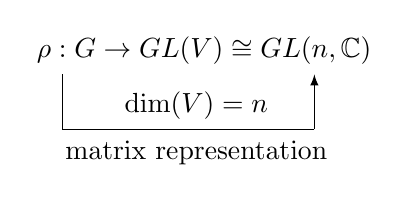
\begin{tikzpicture}
        \node at (1,1.3) {$\rho:G \rightarrow GL(V) \cong GL(n,\mathbb{C})$};
        \node at (0.9,0.6) {$\dim (V) = n$};
        \node at (0.9,0) {matrix representation};
        \draw (-0.8,1) node {} -- (-0.8,0.3) node {};
        \draw (-0.8,0.3) node {} -- (2.4,0.3) node {};
        \draw[-latex] (2.4,0.3) node {} -- (2.4,1) node {};
    \end{tikzpicture}
\end{center}
\begin{definition}
    The \textbf{Character} $\chi_\rho $ of the representation $\rho$, is the function:
    \[\chi_\rho :G\rightarrow \mathbb{C}\]
    \[\chi_\rho(G) = tr \rho(G) = tr A_{\rho(G)}= \sum_{i=1}^n a_{ii}(g) \]
\end{definition}
\par
Some properties:
\begin{enumerate}
    \item $\chi_\rho (1) = \dim(V)$.
    \item $\forall g,h \in G ,\chi_\rho(h) = \chi_\rho(g^{-1}h)g$.
    \item If $\rho$ and $\varphi$ are two isomorphic representations, then $\chi_\rho(g) = 
        \chi_\varphi(g)$.
    \item If $\rho = \rho_1\oplus \cdots \oplus \rho_s $,-direct sum of some (sub) 
        representations, then $\chi_\rho = \sum \chi_{\rho_i} $
    \item $\chi_{\rho\otimes\varphi}(g) = \chi_\rho(g) \cdot \chi_\varphi(g) $
\end{enumerate}
\begin{proof}
    \par
    1. $\rho(1) = E_n$.\ (identical operator, $tr E_n = n$)
    \par
    3. $trA_{\rho(g)} = tr(C^{-1}A_{\rho(g)}C) = trA_{\rho(g)}$. ($C$-transition matrix to a
    new basis)
    \par
    2. $\chi_\rho (g^{-1}hg) = tr A_{\rho(g^{-1})\rho(h)\rho(g)} = trA_{\rho(g^{-1})} 
    trA_{\rho(h)} trA_{\rho(g)} = trA_{\rho(h)}$.
    \par
    4. $V= V_1\oplus \cdots \oplus V_s$
    \par
    In an appropriate basis:
    \[A_\rho(g) = 
    \begin{pmatrix}
        A_{\rho_1(g)}   &       &   0               \\
                        &\ddots &                   \\
        0               &       &   A_{\rho_s(g)}
    \end{pmatrix}
    \Rightarrow trA_{\rho} = \sum_{i=1}^{s} trA_{\rho(g)}
    \]
    \par
    5. Let $(\rho, V)$, $(\varphi, W)$ are representations of the groups $G$, $H$, 
    $(\rho \otimes \varphi, V \otimes W, G \times H)$.
    \par
    $(\rho \otimes \varphi)(g,h)(v_i\otimes w_j) = (\rho(g)v_i)\otimes (\varphi(h)w_j)$.
    Note That for $h = g$, we get a representation of $G$, if:
    \[A = A_{\rho(g)},\ B = A_{\varphi(g)} \Rightarrow\]
    \[A_{\rho \otimes \varphi (g)} = A \times B = 
    \begin{pmatrix}
            a_{11}B & \cdots & a_{1n}B  \\
            \vdots  & \ddots & \vdots   \\
            a_{n1}B & \cdots & a_{nn}B 
    \end{pmatrix}
    \]
    \[tr(A\times B) = \sum_i tr a_{ii}B = trA \cdot trB\]
\end{proof}

%------------------------------------------------------------------------------------------%
\newpage
\section{LECTURE 08 (19.04.2023)}
\subsection{Consequences of Schur's Lemma}
If $\varphi$ is an irreducible representation of $G$ (over $\mathbb{C}$), then its character 
$\chi_\varphi$ is an irreducible character.
\par
(It means that $\chi_\varphi \neq \eta + \theta$, where $\eta , \theta$ are characters.)
\setcounter{lemmacounter}{0}
\begin{lemma}
    \textbf{Schur's Lemma}
    \par
    If $\varphi: G\rightarrow GL(V),\psi :G\rightarrow GL(W)$ are irreducible representations,
    and $f:V\rightarrow W$ is a homomorphism of these representations, then $f=0$, (if $
    \varphi=\psi$), or $f$ is isomorphic. 
\end{lemma}
\textbf{Consequence}: If $K$ is alg closed, $V\equiv W$, $f$ is isomorphism $\Rightarrow f \lambda 
E, \lambda \in K$.
\begin{proof}
    As $K$ is alg closed, then $f: V\rightarrow V \equiv W$ has an eigenvector $v$ with 
    eigenvalue $\lambda$, then the subspace:
    \[V_\lambda = \{v\in V| f(v) = \lambda v\}\neq 0\]
    is an invariant subspace of $V$ $\Rightarrow V_\lambda = V \Rightarrow f = \lambda E$
    is a scalar operator.
\end{proof}
\begin{lemma}
    ($K = \mathbb{C}$) In the condition of \textbf{Schur's Lemma}:
    \par
    Let $f:V\rightarrow W$ be some linear mapping. Consider the average mapping:
    \[
        \widetilde{f}:= \frac1{|G|}\sum_{g \in G} \psi(g)f{\varphi(g)}^{-1} = 
        \begin{cases}
            0,\ if\ \varphi \neq \psi \\
            \lambda,\ if\ V\equiv W,\ \varphi = \psi,\ where\ \lambda = \frac{tr f}{\dim V} 
        \end{cases}
    \]
\end{lemma}
\begin{proof}
    It's evident that:
    $\widetilde{f}\varphi(h) = \psi(h)\widetilde{f} \Rightarrow$ by the Consequence (where 
    $V= W$, $\varphi = \psi$), $\widetilde{f} = \lambda E$, calculate the trace of 
    $\widetilde{f}$:
    \[tr \widetilde{f} = trf = \lambda tr E = \lambda \dim V \]
    \[\lambda = \frac{trf}{\dim V}\]
\end{proof}

\subsection{Matrix Version of the Lemma}
Choose bases in $V$ and $W$:
\[\{v_i|i\in I\subset V\},\ \{w_j|j\in J \subset W \}\]
\par
The matrices of operators are denoted with the same letters
\[\varphi(g) = (\varphi_{ii'}(g)),\ \psi(g) = (\psi_{jj'}(g))\]
\[f = (f_{ji}),\ \widetilde{f} = (\widetilde{f}_{ji})\]
\par
By the definition of $\widetilde{f}$, we can write:
\begin{equation}
    \widetilde{f}_{ji} = \frac1{|G|} \sum_{g,i',j'}\psi_{jj'}(g)f_{j'i'}\varphi_{i'i}(g^{-1})
\end{equation}
\par
If we take $f = E_{j_0i_0}$, $(f_{j_0i_0} = 1,\ f_{ji} = 0,\ if\ (j,i)\neq (j_0,i_0))$
\begin{enumerate}
    \item if $\varphi \neq \psi$, then from (2) $\Rightarrow$
    \begin{equation}
    \frac1{|G|} \sum_{g\in G} \psi_{jj_0}(g)\varphi_{ij}(g') = 0, \forall i, j, i_0,j_0
    \end{equation}
    \item when $V \equiv W$, $\varphi = \psi$, then 
    \[\widetilde{f} = \frac{tr f}{\dim V}E\]
    \[trf = \sum_{i}f_{ii}=\sum_{i,i'}\delta_{j'i} \cdot f_{j'i}'\ \Rightarrow\]
    \[\frac1{|G|}\sum \varphi_{jj'}(g)\cdot f_{j'i}\cdot \varphi_{i'i}(g^{-1})
    = \frac{\delta_{ji}}{\dim V}\sum_{j',i'}\delta_{j'i'}\cdot f_{j'i'} \]
    Taking $f = E_{j_0i_0}$, we got:
    \[
        \frac1{|G|}\sum_{g\in G}\varphi_{jj_0}(g)\varphi_{i_0i}(g^{-1}) = 
        \begin{cases}
            \frac{\delta_{ji}}{\dim V}, if\ i_0 = j_0, \\
            0,\ otherwise
        \end{cases}
    \]
\end{enumerate}

\subsection{Orthogonality relation of characters}
\begin{definition}
    Define on the space $F_G$ of all functions $f:G\rightarrow \mathbb{C}$, the Hermitian 
    scalar product: 
    \[{(f_1, f_2)}_G := \frac1{|G|}\sum_{g\in G} f_1(g)\overline{f_2(g)}\]
\end{definition}
\par
If $\chi, \theta$ are characters, then they are constant on conjugate classes, if $G = 
\bigcup_{i=1}^{r} K_i, (K_1\ldots K_r)$ are all conjugate classes, so
\[{(\chi,\theta)}_G = \frac1{|G|}\sum_{i=1}^{r}|K_i|\chi(g_i)\theta(g_i),\ when\ g_i\in K_i\]
\begin{theorem}
    (The first orthogonality relation) Let $\varphi, \psi$ are irreducible Representations
    of $G$ over $\mathbb{C}$
    \[\frac1{|G|}\sum_{g\in G} \psi_{jj_0}(g)\varphi_{i_0i}(g^{-1}) = 0,\ \forall i,j,i_0,
    j_0 \]
    then 
    \[
        (\chi_\varphi, \chi_\psi) = \delta_{\varphi,\psi} = 
        \begin{cases}
            1,\ if\ \varphi \neq \psi, \\
            0,\ otherwise.
        \end{cases}
    \]
\end{theorem}
\begin{proof}
    $\chi_{\varphi(g)} = \sum_i\varphi_{ii}(g)$, $\chi_{\psi(g)} = \sum\psi_{jj}(g)$.
    Put  $i = i_0j = j_0$ and sum over all $i,j \Rightarrow$
    \[
        \frac1{|G|}\sum_{g,i,j}\psi_{ij}(g)\varphi_{ji}(g^{-1}) = \frac1{|G|}\sum_{g\in G}
        \psi_{ij}(g)\varphi_{ji}(g^{-1}) = {(\chi_\psi,\chi_\varphi)}_G
    \]
\end{proof}
\par
\textbf{Consequence 1}: The number $s$ of all pairwise non-isomorphic irreducible complex
representations of $G$, $s = r$ -the number of conjugate classes of $G$.
\begin{proof}
    The irreducible characters $\chi_{1}\ldots\chi_{s}$ are orthogonal $\Rightarrow$ they
    are linearly independent, but $\dim ZF(G)$ (the space of central class) functions on 
    $G$, which are constant on conjugate classes.
    \par
\end{proof}

%------------------------------------------------------------------------------------------%
\newpage
\section{LECTURE 9 (26.04.2023)}
%------------------------------------------------------------------------------------------%
\newpage
\section{LECTURE 10 (03.05.2023)}
%------------------------------------------------------------------------------------------%
\newpage
\appendix
\section{Sylow Theorems}
Sylow Theorems\cite{milneGT}
%------------------------------------------------------------------------------------------%
\newpage
\bibliographystyle{plain}
\clearpage
\addcontentsline{toc}{section}{Reference}
\bibliography{Reference}
\end{document}